
\chapter{Protezione}
\section{Introduzione}
\paragraph{Premessa} \[\boxed{\text{Il meccanismo di protezione non nasce per difendersi dagli hacker.}}\]
\paragraph{Come nasce l'idea} La necessità della protezione nasce dall'utilizzo dei grandi calcolatori degli anni $60$ per eseguire più programmi contemporaneamente. 
\begin{enumerate}
	\item L'utente richiede l'utilizzo del calcolatore lasciando il suo codice.
	\item Gli operatori inseriscono il codice nel calcolatore (pensare alla \emph{Calcolatrice Elettronica Pisana}) e lo eseguono.
	\item L'utente ritira dopo un po' di tempo l'output del programma lasciato.
\end{enumerate}
Abbiamo un \emph{batch processing}. Devo caricare programmi complessi, con molti dati che potrebbero provocare tempi di attesi lunghi prima dell'esecuzione: l'idea è che mentre attendo passo a occuparmi di un altro programma da eseguire. Chiaramente posso fare una cosa di questo tipo solo col meccanismo delle interruzioni: al termine del caricamento dei dati lancio un'interruzione. 
\paragraph{Quanto fatto fino ad ora non basta} Le istruzioni che abbiamo visto fino ad ora (relative alle interruzioni) possono essere eseguite senza problemi, dunque un programma potrebbe interferire con il meccanismo delle interruzioni. Il programma può dare fastidio in vari modi (per esempio con istruzioni mov che modificano il codice del programma).
\paragraph{Soluzione} La soluzione al problema è di tipo hardware, non possiamo fare diversamente. Dobbiamo distinguere due modalità per il processore:
\begin{itemize}
	\item \textbf{modalità sistema}, destinata al codice dell'operatore (nessun limite di esecuzione);
	\item \textbf{modalità utente}, destinata al codice degli utenti (non è ammessa l'esecuzione di tutte le istruzioni, o l'esecuzione di operazioni di scrittura/lettura in certe aree di memoria).
\end{itemize}
Dobbiamo prevedere meccanismi che permettono il passaggio da una modalità all'altra. In alcuni casi vengono implementate più modalità: avere più livelli di privilegio è una questione di efficienza, cose che non ci interessano.
\paragraph{Memoria} Nella memoria di sistema abbiamo il codice stabilito dagli operatori, ma anche i codici dei vari \emph{job} da eseguire. Ogni tanto si salta al codice degli operatori:
\begin{enumerate}
	\item interruzione esterna,
	\item eccezione,
	\item l'utente ha esplicitamente invocato una routine del sistema.
\end{enumerate}
In tutti e tre i casi vogliamo che il processore si porti in modalità sistema. La cosa più semplice è associare anche il terzo elemento alle interruzioni. Possiamo invocare una routine del sistema con la seguente istruzione
\begin{verbatim}
	INT $tipo
\end{verbatim}
L'innalzamento del livello di privilegio non può che passare dall'IDT.
\paragraph{Codice del kernel} Ci dovrebbe preoccupare che il codice dell'operatore sia, adesso lo possiamo dire, il codice del kernel? 
\begin{itemize}
	\item L'area di memoria con questo codice NON deve essere accessibile a programmi eseguiti in modalità utente. Gli utenti, come già anticipato, \textbf{NON} devono avere libero accesso a tutta la memoria!
\end{itemize}
\paragraph{Modalità utente} In una modalità privilegiata esistono limiti su:
\begin{itemize}
	\item istruzioni eseguibili (si distinguono quelle eseguibili, \emph{privilegiate}, da quelle eseguibili, \emph{non privilegiate});
	\item indirizzi a cui si può accedere (operazioni di lettura e scrittura).
\end{itemize}
Il processore in modalità utente non esegue istruzioni privilegiate e non accede a indirizzi dove non può accedere: se gli si chiede di fare queste cose genera un'\emph{eccezione di protezione}. Queste cose limitano l'utente su tutti e tre gli elementi fondamentali dell'architettura di un elaboratore: CPU (limitano il controllo della CPU impedendo l'esecuzione di particolari istruzioni), la RAM e l'I/O (non tutti gli indirizzi sono accessibili). 
\paragraph{Motivazioni} Abbiamo già detto che la questione non è proteggersi dagli hacker, ma proteggere un utente da un altro, impedire a un utente di proseguire il suo lavoro a causa di un altro utente (\emph{la polizia, che protegge i cittadini da altri cittadini}, cit.). 
\begin{framed}\noindent\textbf{Regola base per ogni cosa che gestiamo} Quando siamo in modalità sistema non possiamo fidarci di ciò che potrebbe essere stato gestito in modalità utente. Dobbiamo pensare all'utente come una persona che farà tutto in suo potere per sovvertire il sistema.
\end{framed}\paragraph{Modalità del processore all'avvio} All'avvio del sistema siamo in modalità sistema. Ecco perché in QEMU siamo liberi di fare ciò che ci pare! 
\section{Protezione nel processore Intel} L'Intel ha introdotto la protezione nel 286 (a 16 bit), un sistema derivato da \emph{multics} (\emph{Multiplexer information and communication system}), un sistema operativo sviluppato da MIT e \emph{Bell Labs}. Questo sistema operativo possedeva diversi livelli di privilegio: l'Intel introdusse un architettura segmentata, meccanismo di cui dobbiamo tenere conto.

\paragraph{Cosa si intende con architettura segmentata?} Divido la memoria in più segmenti (codice, dati). Ogni volta che si deve riferire un certo byte bisogna specificare sia il segmento che ci interessa che l'offset all'interno del segmento. La cosa, su cui Intel ha insistito, non è risultata popolare: l'architettura a cui noi siamo abituati è un architettura \emph{flat}.


\paragraph{Approfondiamo i meccanismi} Il meccanismo dell'Intel è abbastanza elaborato: fa tante cose, tutte importanti (\underline{dobbiamo imparare un po' a memoria}, cit.). Vediamo più nel dettaglio...
\subsection{Livello di privilegio attuale del processore (\emph{Current Privilege Level})} 
All'interno del processore Intel è presente un registro CS (\emph{Code Selector}) che contiene negli ultimi due bit il livello di privilegio e l'identificatore del segmento codice corrente. La segmentazione non ci interessa, dunque guarderemo solo i primi due bit (che definiamo CPL, \emph{Current Privilege Level}). I valori possibili sono 
\begin{multicols}{2}
	\begin{itemize}
		\item $00$ (sistema), e
		\item  $01$ (utente).
	\end{itemize}
\end{multicols}
\subsection{Protezione e interruzioni, cambi di modalità (gate e IRETQ)} L'altra cosa su cui si basa l'architettura Intel è l'associare tutti i possibili cambi di livelli di privilegio al meccanismo delle interruzioni.
\begin{itemize}
	\item Il passaggio dal gate può avvenire solo attraverso un'interruzione esterna, un'interruzione interna o l'esecuzione dell'istruzione INT. Il livello di privilegio successivo al passaggio del gate deve essere maggiore o uguale: non è possibile che un calcolatore in modalità sistema si ritrovi in modalità utente dopo aver attraversato il gate, al più si ritrova nella stessa modalità. 
	\item L'istruzione IRETQ confronta il vecchio CPL col nuovo e permette solo passaggi con livello di privilegio minore o uguale rispetto a quello corrente: sono possibili passaggi da modalità sistema a modalità utente, ma non il contrario. 
\end{itemize}
\begin{center}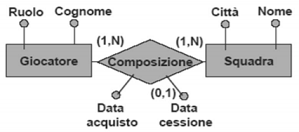
\includegraphics[scale=.75]{img/120.PNG}\end{center}

\subsubsection{Contenuto del gate e \emph{Global Descriptor Table}}  	
\begin{itemize}
	\item All'interruzione abbiamo sempre associato un tipo: in alcuni casi è stabilito dall'APIC (interruzioni esterne), in altri dall'operando di una istruzione (istruzione INT), in altri ancora è implicito (eccezioni).
	\item Il tipo permette di identificare un'entrata dell'IDT. Ciascuna entrata contiene delle informazioni. Quelle che ci interessano maggiormente sono:
	\begin{itemize}
		\item l'indirizzo della routine da mandare in esecuzione (nulla di nuovo);
		\item un bit I/T che indica il tipo del gate (\textit{interrupt} o \textit{trap}, nulla di nuovo);
		\item un flag $P$, che specifica se la routine è stata implementata o no;
		\begin{itemize} 
			\item Logicamente non saranno implementate tutte le 256 routine possibili.
			\item Se $P=0$ il processore non può attraversare il \emph{gate} e genera una nuova eccezione di tipo \emph{gate non implementato}. I programmatori di sistema solitamente implementano questa eccezione: se ciò non avviene il processore subisce una doppia eccezione (\emph{abort}) e si spegne. 
		\end{itemize}
		\item il \emph{Descriptor Privilege Level}, che indica il livello di privilegio minimo  che il processore deve avere prima di attraversare un certo gate;
		\begin{itemize}
			\item Notare che \textbf{con un'interruzione esterna e un'eccezione il gate viene attraversato comunque}, la limitazione sta solo nell'uso dell'istruzione INT. La cosa è utile per prevenire l'esecuzione attraverso INT di routine normalmente associate a interruzioni esterne e/o eccezioni.
		\end{itemize} 
		\item Un selettore di codice relativo a un'entrata della \emph{Global Descriptor Table}, quella del segmento dove si trova la routine.
	\end{itemize}
\end{itemize} 

\paragraph{A cosa ci serve il selettore di codice?} Per trovare il livello di privilegio dopo aver attraversato il gate. Detto in altro modo: cosa dobbiamo scrivere nel \emph{Current Privilege Level} dopo aver attraversato il gate?
\begin{itemize}
	\item  L'informazione non si trova nella tabella delle interruzioni ma nella \emph{Global Descriptor Table} (GDT), tabella legata al meccanismo della segmentazione. La tabella, dato il segmento codice dove si trova la routine, indica una serie di informazioni:
	\begin{itemize}
		\item da che indirizzo parte;
		\item quanto è grande il segmento;
		\item \textbf{il livello di privilegio}!
	\end{itemize} 
	\item Il meccansimo della Intel è flessibile: si da la possibilità di decidere se innalzare o no il livello di privilegio: ciò per noi è una semplice constatazione, innalzeremo sempre il livello di privilegio.
\end{itemize} 
%\paragraph{Come raggiungiamo la relativa entrata nella GDT?} Nella IDT troviamo il relativo selettore di codice (\emph{code selector}) relativo al segmento di codice dove si trova la routine.
\clearpage
\subsubsection{Necessità di una nuova pila}
Alcune informazioni vengono memorizzate in pila. Non possiamo utilizzare in modalità sistema il contenuto di una pila manipolato dall'utente (non possiamo fidarci dell'utente, MAI). Segue la necessità di fare un cambio di pila qualora vi sia un cambio di privilegio.\begin{itemize}
	\item Distinguiamo due pile: la \emph{pila utente} e la \emph{pila sistema}.
	\item \textbf{Se il livello di privilegio si innalza il processore passa da pila utente a pila sistema} (si confronta il \emph{Current Privilege Level} col nuovo livello di privilegio trovato nella \emph{Global Descriptor Table}). Cambiare pila significa modificare il valore del registro RSP. Nella pila sistema andiamo a porre delle informazioni: 
	\begin{center}
		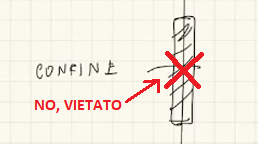
\includegraphics[scale=.8]{img/283.PNG}
	\end{center}
	\begin{enumerate}
		\item il vecchio RIP.
		\item il vecchio registro CS (in particolare il vecchio CPL);
		\item i vecchi flag (RFLAGS);
		\item il vecchio RSP (cioè dov'era RSP prima di fare il passaggio);
		\item il selettore pila vecchio (che non ci interessa poichè legato alla segmentazione);
	\end{enumerate}
	queste informazioni rendono possibile il ritorno nella pila utente.
	\item Salvate tutte queste informazioni il processore preleva dal gate il nuovo RIP e il nuovo CS (in particolare il nuovo CPL). 
	\item La IRETQ confronta il \emph{Current Privilege Level} e il CPL preso dal vecchio valore di CS in pila. Per prima cosa si verifica che il vecchio valore sia al più uguale (e non maggiore) del CPL attuale (controllo necessario per impedire violazioni del meccanismo della protezione\footnote{L'utente potrebbe fare casini modificando RSP prima di lanciare la IRETQ.}). Successivamente si verifica se è necessario riportare in RSP la pila utente (confronto tre \emph{Current Privilege Level} e il CPL preso dal vecchio valore di CS in pila). La IRETQ ripristina ciò che va ripristinato recuperando le informazioni dalla pila corrente (quella puntata con RSP). 
\end{itemize}
\paragraph{Osservazione} \emph{pushf} e \emph{popf} non permettono l'alterazione di tutti i flag. Abbiamo visto che per modificare il trap flag utilizziamo una funzione con istruzioni \emph{pushf} e \emph{popf}. Quindi è possibile modificare qualunque flag in questo modo? No, \emph{iretq} e \emph{popf} non permettono la sovrascrizione di tutti i flag: contrariamente ad altre situazioni non si ha un'eccezione, semplicemente si ignorano le richieste di modifica senza effetti visivi.

\subsubsection{Da dove viene preso il puntatore alla nuova pila?} 
L'Intel nel 286 prevedeva la possibilità di gestire la microprogrammazione quasi completamente in hardware (anche questa cosa sostanzialmente non usata). Dai GDT è possibile raggiungere i \emph{Task State Segment} (TSS). Questi segmenti, previsti di suo dal processore Intel e identificati da una certa entrata della GDT, contengono informazioni relative a un particolare programma in esecuzione. Inoltre si ha un registro \emph{Task Register} (TR) contenente l'indice del \emph{task/job} corrente. Nel TSS si hanno tante informazioni, tra queste \textbf{il puntatore \underline{alla base} della pila sistema}. 
\begin{center}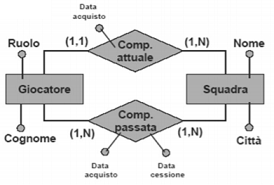
\includegraphics[scale=.75]{img/121.PNG}\end{center}
Quando c'è un'interruzione il processore usa TR per accedere al segmento TSS a partire dalla GDT, trovando così l'indirizzo della pila sistema.


\subsection{Livello di privilegio e istruzioni IN/OUT/CLD/STD (flag IOPL)}
Le istruzioni IN/OUT/CLD/STD non sono automaticamente vietate a livello utente. Esiste un altro campo, nel registro dei flag, detto \emph{IO Privilege Level} (IOPL), che per noi assume come valore 
\begin{multicols}{2}
	\begin{itemize}
		\item $00$ (sistema) o
		\item $11$ (utente).
	\end{itemize} 
\end{multicols} \noindent Con questo definiamo il livello privilegio che dobbiamo avere per eseguire le istruzioni IN/OUT/CLD/STD. L'informazione è statica e rimane lì anche dopo passaggi di gate. Le modifiche al campo sono ignorate nell'esecuzione di POPF e IRETQ. 

\subsection{Morale della favola}
\begin{framed}
	\noindent Per far funzionare le interruzioni abbiamo bisogno di:
	\begin{itemize}
		\item almeno un segmento TSS (ci serve un solo TSS per gestire i passaggi tra due livelli di privilegio),
		\item almeno un descrittore nella GDT,
		\item e il registro TR inizializzato in modo da contenere l'identificativo di questo descrittore. 
	\end{itemize}  Fortunatamente possiamo fare questa cosa all'avvio.
\end{framed}
\clearpage

\section{Esempio di programma: passaggio a livello utente (\emph{liv$\_$utente})}
\paragraph{Perchè ci interessa questa cosa?} Il nostro programma parte in modalità sistema, a un certo punto vogliamo passare in modalità utente. La IRETQ da sola non basta, dobbiamo impostare la pila nei modi detti prima per compiere il cambio di privilegio.
\paragraph{Esempio} Supponiamo di voler eseguire la seguente funzione due volte: la prima volta in modalità sistema e la seconda in modalità utente.
\begin{verbatim}
	void foo() {
		natb c;
		printf("Provo a leggere RBR\n");
		c = inputb(0x60);
		printf("Ho letto RBR: %2x\n", c);
	}
\end{verbatim}
Gestiamo il passaggio a livello utente attraverso la funzione \emph{liv$\_$utente}, che poniamo nel nostro codice tra le due chiamate di \emph{foo}.
\begin{verbatim}
	foo();
	liv_utente();
	foo();
\end{verbatim}
\begin{center}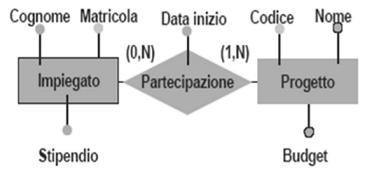
\includegraphics{img/122.PNG}\end{center}
La funzione si bassa sulla necessità di passare dalla IRETQ per effettuare un passaggio da modalità sistema a modalità utente. Sappiamo che la IRETQ recupera del contenuto dalla pila e lo utilizza: segue che per utilizzare la IRETQ dovremo mettere in pila ciò che la funzione si aspetta. Le cose sono quelle già elencate prima
\begin{enumerate}
	\item Tolgo l'indirizzo di ritorno con la pop
	\item Pongo il selettore dati utente (il vecchio contenuto del registro SS, non ci interessa)
	\item Pongo l'RSP
	\item Pongo il registro dei flag aggiornato
	\item Pongo il selettore codice utente (il contenuto del registro CS, ci interessa il CPL)
	\item Pongo l'indirizzo di ritorno rimosso all'inizio
	\item Chiamo la IRETQ
\end{enumerate}
\begin{center}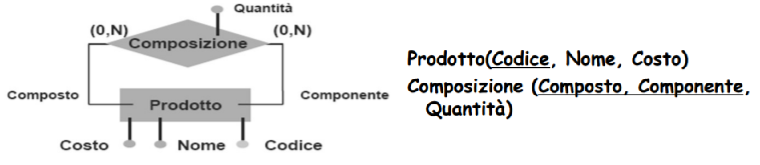
\includegraphics{img/123.PNG}\end{center}
A questo punto ogni istruzione che richiede un livello di privilegio maggiore rispetto a quello corrente provocherà il lancio di un'eccezione di tipo 13 (\emph{eccezione di protezione}). L'eccezione è di tipo \emph{fault}, dunque l'indirizzo stampato del warming è quello dell'istruzione che ha causato il problema (la IN). 